% !TEX TS-program = pdflatex
% !TEX encoding = UTF-8 Unicode

% This is a simple template for a LaTeX document using the "article" class.
% See "book", "report", "letter" for other types of document.

\documentclass[11pt]{article} % use larger type; default would be 10pt

\usepackage[utf8]{inputenc} % set input encoding (not needed with XeLaTeX)

%% Examples of Article customizations
% These packages are optional, depending whether you want the features they provide.
% See the LaTeX Companion or other references for full information.

%% PAGE DIMENSIONS
\usepackage{geometry} % to change the page dimensions
%\geometry{letterpaper} % or letterpaper (US) or a5paper or....
 \geometry{margin=1in} % for example, change the margins to 2 inches all round
% \geometry{landscape} % set up the page for landscape
%   read geometry.pdf for detailed page layout information

\usepackage{graphicx} % support the \includegraphics command and options

% \usepackage[parfill]{parskip} % Activate to begin paragraphs with an empty line rather than an indent

%% PACKAGES
\usepackage{listings}
\usepackage{booktabs} % for much better looking tables
\usepackage{array} % for better arrays (eg matrices) in maths
\usepackage{paralist} % very flexible & customisable lists (eg. enumerate/itemize, etc.)
\usepackage{verbatim} % adds environment for commenting out blocks of text & for better verbatim
%\usepackage{subfig} % make it possible to include more than one captioned figure/table in a single float
% These packages are all incorporated in the memoir class to one degree or another...
\usepackage[usenames,dvipsnames]{color}
\usepackage{caption}
\usepackage{subcaption}
\usepackage{float}
%% HEADERS & FOOTERS
\usepackage{fancyhdr} % This should be set AFTER setting up the page geometry
\pagestyle{fancy} % options: empty , plain , fancy
\renewcommand{\headrulewidth}{0pt} % customise the layout...
\lhead{}\chead{}\rhead{}
\lfoot{}\cfoot{\thepage}\rfoot{}

% paragraph indent http://tex.stackexchange.com/questions/45501/how-to-add-indentation
\usepackage{indentfirst}

%% SECTION TITLE APPEARANCE
\usepackage{sectsty}
\allsectionsfont{\sffamily\mdseries\upshape} % (See the fntguide.pdf for font help)
% (This matches ConTeXt defaults)

%% ToC (table of contents) APPEARANCE
\usepackage[nottoc,notlof,notlot]{tocbibind} % Put the bibliography in the ToC
\usepackage[titles,subfigure]{tocloft} % Alter the style of the Table of Contents
\renewcommand{\cftsecfont}{\rmfamily\mdseries\upshape}
\renewcommand{\cftsecpagefont}{\rmfamily\mdseries\upshape} % No bold!

%% END Article customizations
%%code listings settings
%%http://stackoverflow.com/questions/3175105/how-to-insert-code-into-a-latex-doc
\usepackage{color}

\definecolor{dkgreen}{rgb}{0,0.6,0}
\definecolor{gray}{rgb}{0.5,0.5,0.5}
\definecolor{mauve}{rgb}{0.58,0,0.82}


\lstset{frame=tb,
	language=Verilog,
	aboveskip=3mm,
	belowskip=3mm,
	showstringspaces=false,
	columns=flexible,
	basicstyle={\small\ttfamily},
	numbers=none,
	numberstyle=\tiny\color{gray},
	keywordstyle=\color{blue},
	commentstyle=\color{dkgreen},
	stringstyle=\color{mauve},
	breaklines=true,
	breakatwhitespace=true,
	tabsize=3
}

%% The "real" document content comes below...

\title{
	{\Huge Team 2 Goofy Lights Editor}
	\\
	{\Large CS-383}}
\author{
	\\
	\makebox[.3\linewidth]{Nick Krenowicz}\\Program Flow Leader\ \and
	\\
	\makebox[.3\linewidth]{Paul Martin}\\GUI Leader\ \and
	\\
	\makebox[.3\linewidth]{Tim Sonnen}\\File Master\ \and
	\\
	\makebox[.3\linewidth]{Kevin Dorscher}\\Linked List / Developer\ \and
	\\
	\makebox[.3\linewidth]{Joe Carter}\\Developer\ \and
	\\
	\makebox[.3\linewidth]{Lise Welch}\\Developer\ \and
	\\
	\makebox[.3\linewidth]{Emma Bateman}\\Developer\ \and
	\\
	\makebox[.3\linewidth]{Bruce Bolden}\\Inspirational Teacher\ %empy spaceholder to bump emma left
	\\
	\\
	\\
	\\}
	 
	%Nick Krenowicz -- Program Flow Leader \\
	%Paul Martin -- QT/GUI Leader\\ 
	%Tim Sonnen -- File Master \\
	%Kevin Dorscher -- Linked List Librarian \\
	%Joe Carter -- Developer \\
	%Lise Welch -- Developer \\
	%Emma Bateman -- Developer \\
	%\\
\date{\today} % Activate to display a given date or no date (if empty),
         % otherwise the current date is printed 

\begin{document}
\lstset{language=C++}
\maketitle
\pagebreak

\tableofcontents


\section{About this Project}
This project is a alteration of the Tower Lights Project done in previous semesters for Cs 383 at the University of Idaho. The end goal of this project is to create an editor for the Goofy Glasses. goofy glasses are a creation of the University of Idaho computer science department, goofy glasses are normal sun glasses, with RGB LED lighting, and a transmitter to send and receive data to turn the LED's on each pair of glasses on or off, as well as change the color the glasses are currently displaying. The editor we (team 2) are creating will be able to set specific coloring patterns for all of the goofy glasses at once. The general idea behind this is to create a grid with individual squares, where each square represents a single pair of goofy glasses. The user will then be able to create frames, and make a slide show of frames, and transmit the data from the slide show to the goofy glasses to create a scene. 

\subsection{Design process}
The general outline of the development process can be simplified into three basic steps. Our first order of business was to start developing back-end functionality for the use cases specified (see appendix). Secondly, we created a basic GUI template to visualize layout, and speculate where extra functionality may be needed. Lastly, our focus was placed on integrating the back-end functionality we created with the GUI to bring everything together.

\section{Sprint 1 \& 2}
\subsubsection{Problems encountered}
Some of the issues we have encountered as a team are presented below. Originally we created a set of global variables, that almost every function would need access to such as, row\#, col\#, and RGB data. This worked great for testing purposes, but has created scoping issues for future updates. We are currently working on changing all of the global variables previously mentioned into local variables. We are currently working on altering our existing functions to deal with this scope change from global to local. We also originally created a RGB type, and are now altering this to an already existing Qt RGB type called Qcolor. Lastly, we are currently considering data flow, and how data will be used be in our goofy lights editor, we have discussed creating some data flow diagrams to help visualize this process.




\subsection{Figures}
\subsubsection{Gui Screenshots}
  
  \begin{figure}[H]
  	\centering
  	\fbox{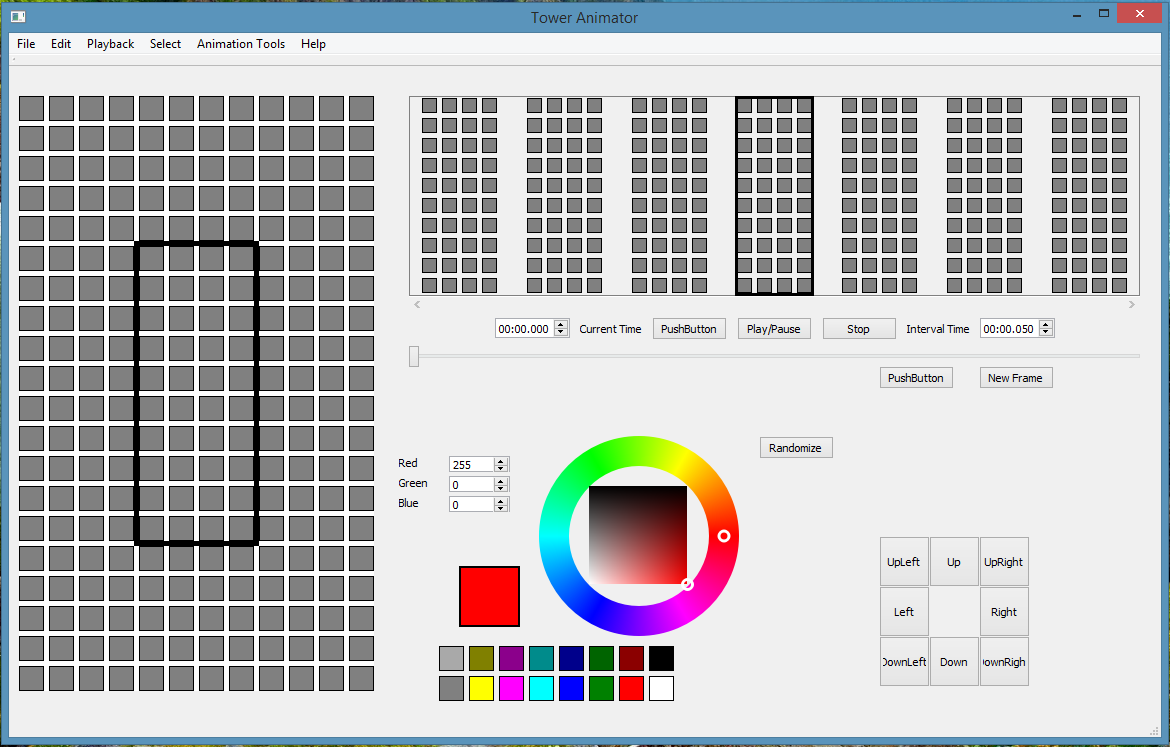
\includegraphics[width=350pt]{GUI_Screenshots/Previous_TowerAnimatorScreenShot.png}}
  	\caption{Original GUI design from previous tower lights project}
  	\label{fig:GUI Base Design Reference}
  \end{figure}
  
  
  \begin{figure}[H]
  	\centering
  	\fbox{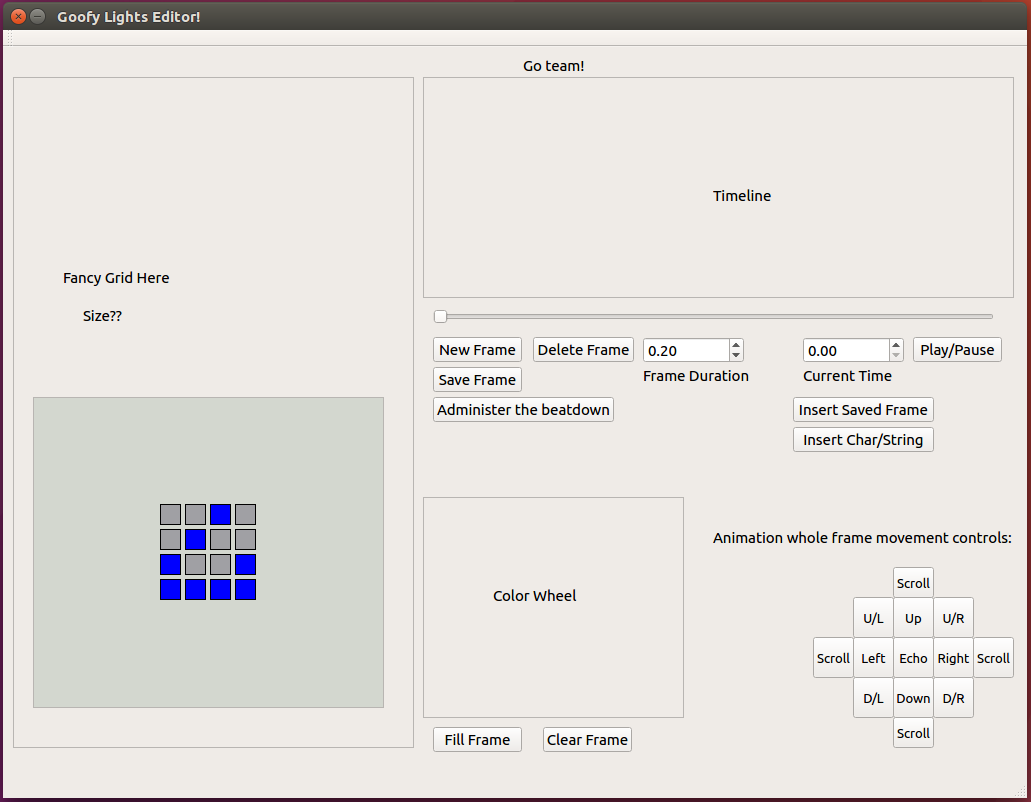
\includegraphics[width=320pt]{GUI_Screenshots/gui_1.png}}
  	\caption{Our initial GUI after first sprint}
  	\label{fig:GUI Design 1}
  \end{figure}
  
  \begin{figure}[H]
  	\centering
  	\fbox{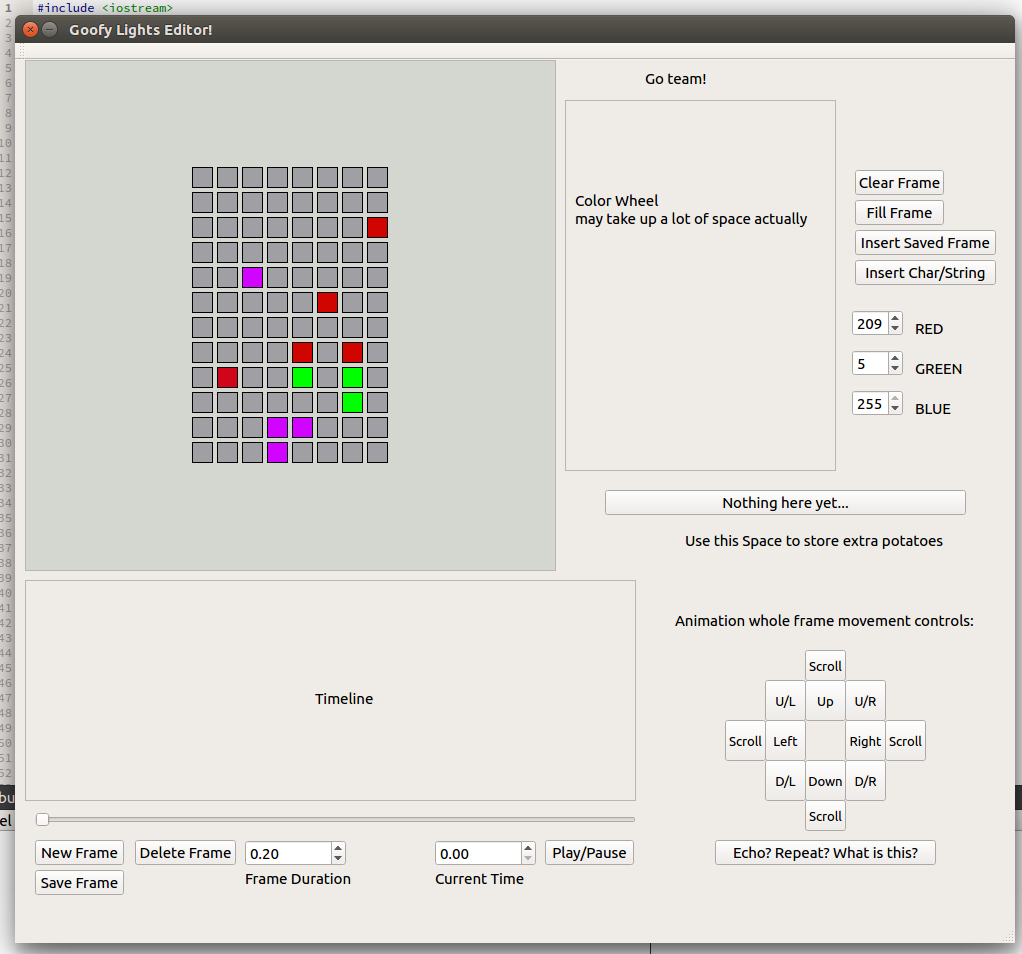
\includegraphics[width=320pt]{GUI_Screenshots/gui_2.png}}
  	\caption{GUI after second sprint, RGB functionality added}
  	\label{fig:GUI Design 2}
  \end{figure}  
  
  \begin{figure}[H]
  	\centering
  	\fbox{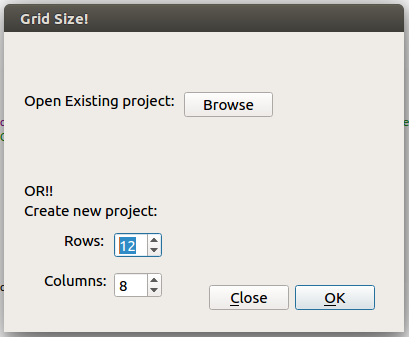
\includegraphics[width=320pt]{GUI_Screenshots/gui_2_dialog.png}}
  	\caption{Grid size selection dialog added}
  	\label{fig:GUI Design 2 dialog}
  \end{figure}
  
  \begin{figure}[H]
  	\centering
  	\fbox{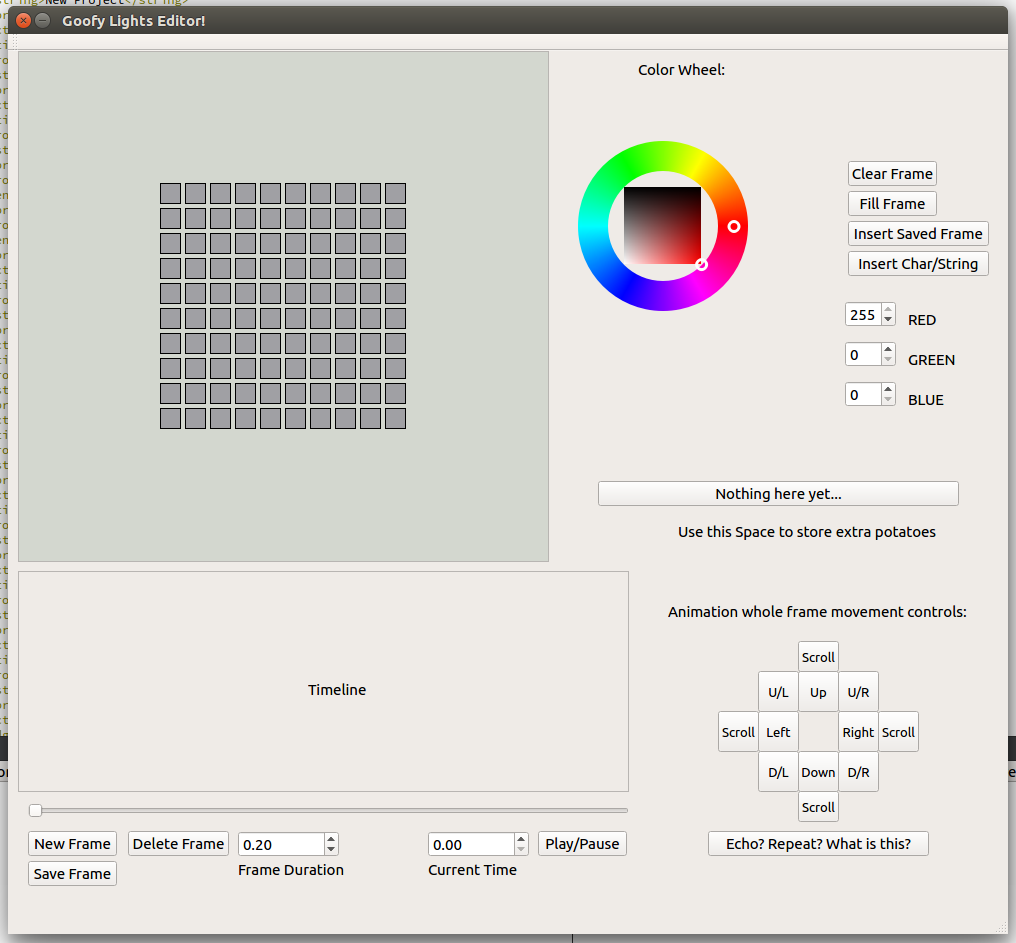
\includegraphics[width=320pt]{GUI_Screenshots/gui_3_1.png}}
  	\caption{Color wheel added in sprint 3}
  	\label{fig:GUI Design 3}
  \end{figure}
  
  \begin{figure}[H]
  	\centering
  	\fbox{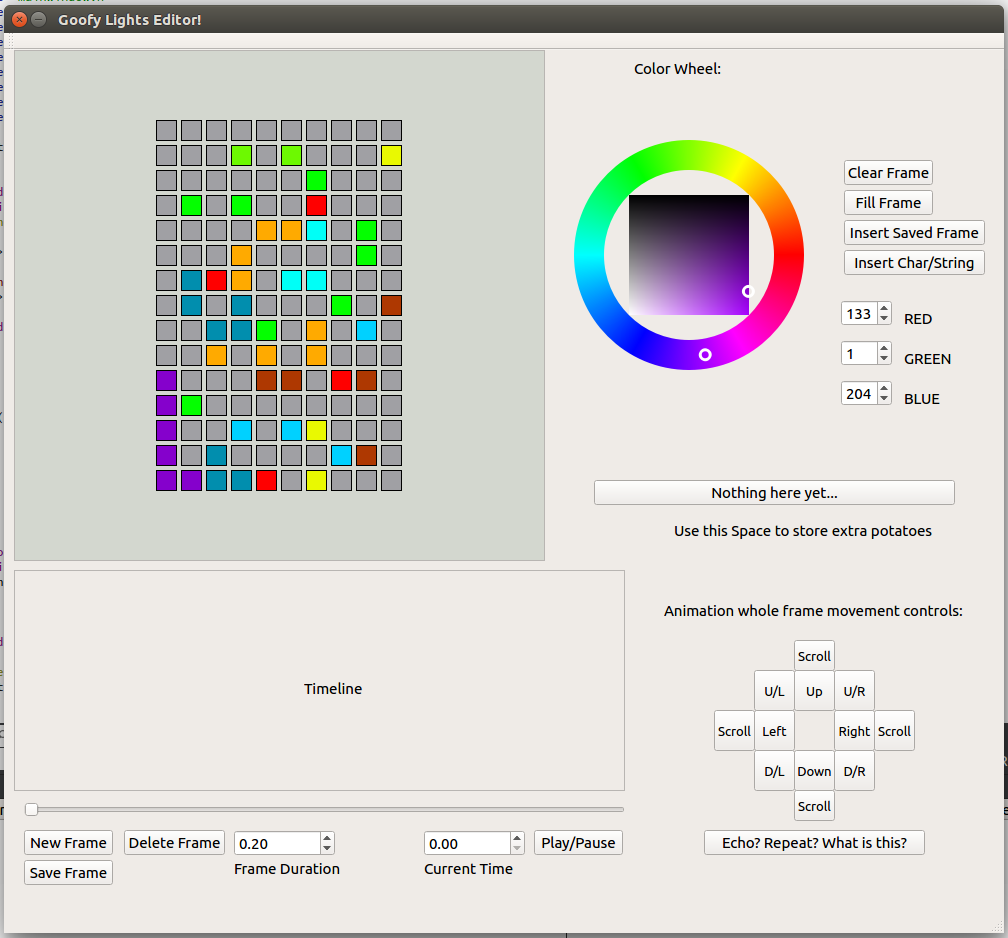
\includegraphics[width=305pt]{GUI_Screenshots/gui_3_2.png}}
  	\caption{Color wheel demo}
  	\label{fig:GUI Design 3 demo}
  \end{figure}
  
  \begin{figure}[H]
  	\centering
  	\fbox{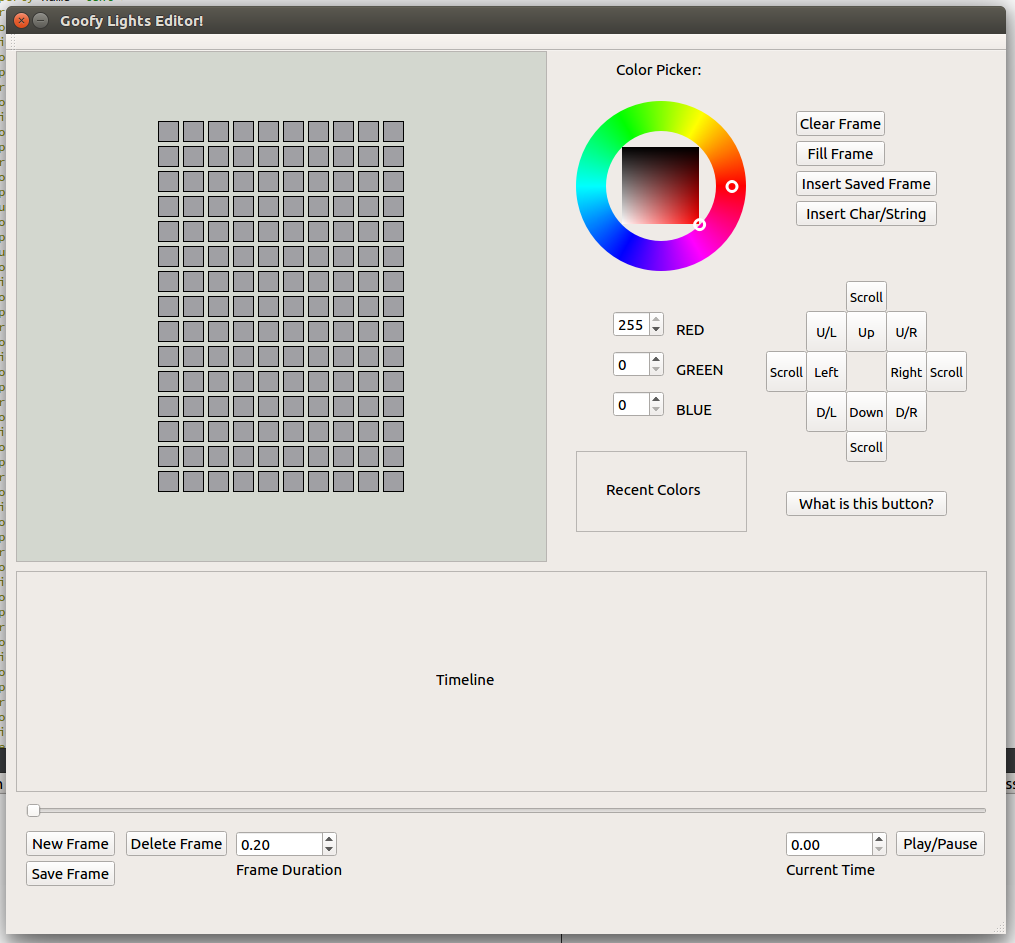
\includegraphics[width=305pt]{GUI_Screenshots/gui_4.png}}
  	\caption{Control buttons moved in sprint 3}
  	\label{fig:GUI Design 4}
  \end{figure}
  
  \begin{figure}[H]
  	\centering
  	\fbox{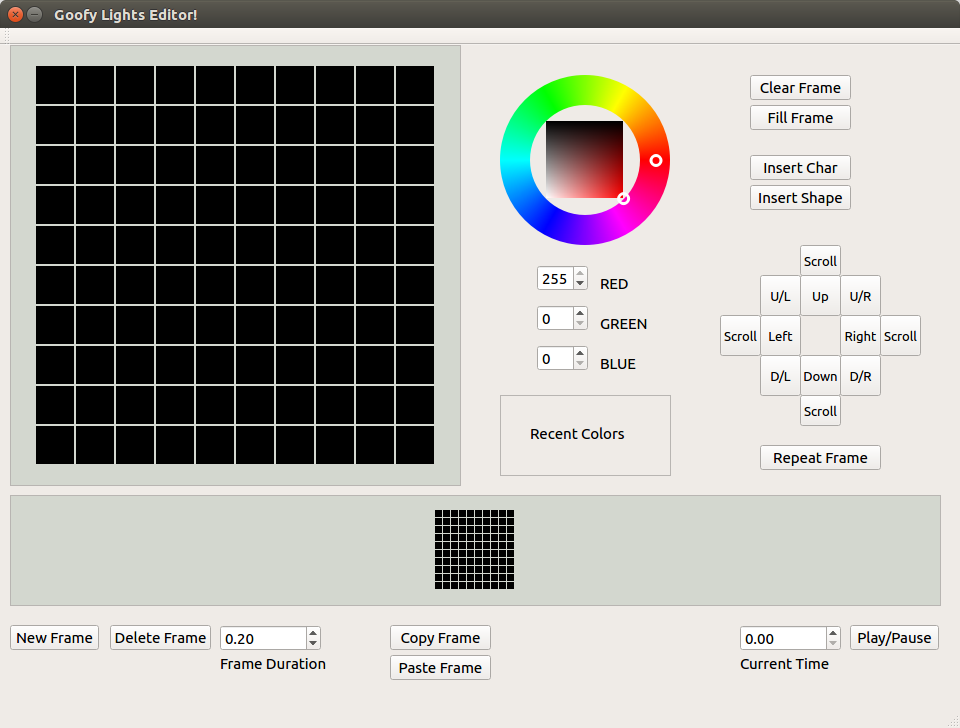
\includegraphics[width=320pt]{GUI_Screenshots/gui_5_1.png}}
  	\caption{Timeline implemented. Default squares now black}
  	\label{fig:GUI Design 5}
  \end{figure}  
  
  \begin{figure}[H]
  	\centering
  	\fbox{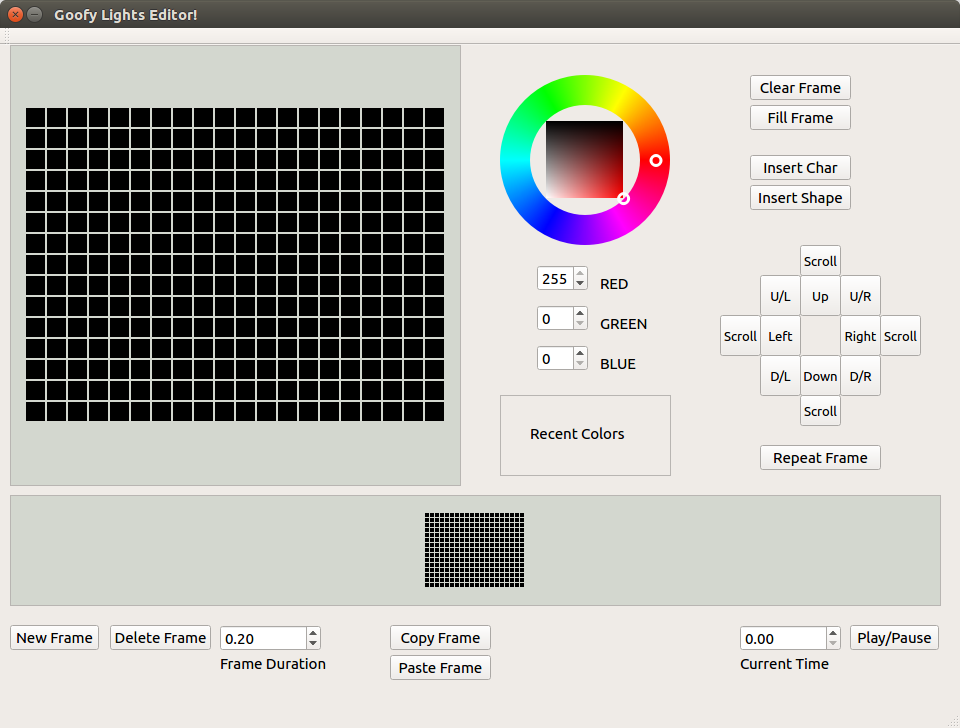
\includegraphics[width=320pt]{GUI_Screenshots/gui_5_3.png}}
  	\caption{Grid size demo 15x20}
  	\label{fig:GUI Design 5 size demo 1}
  \end{figure} 
  
  \begin{figure}[H]
  	\centering
  	\fbox{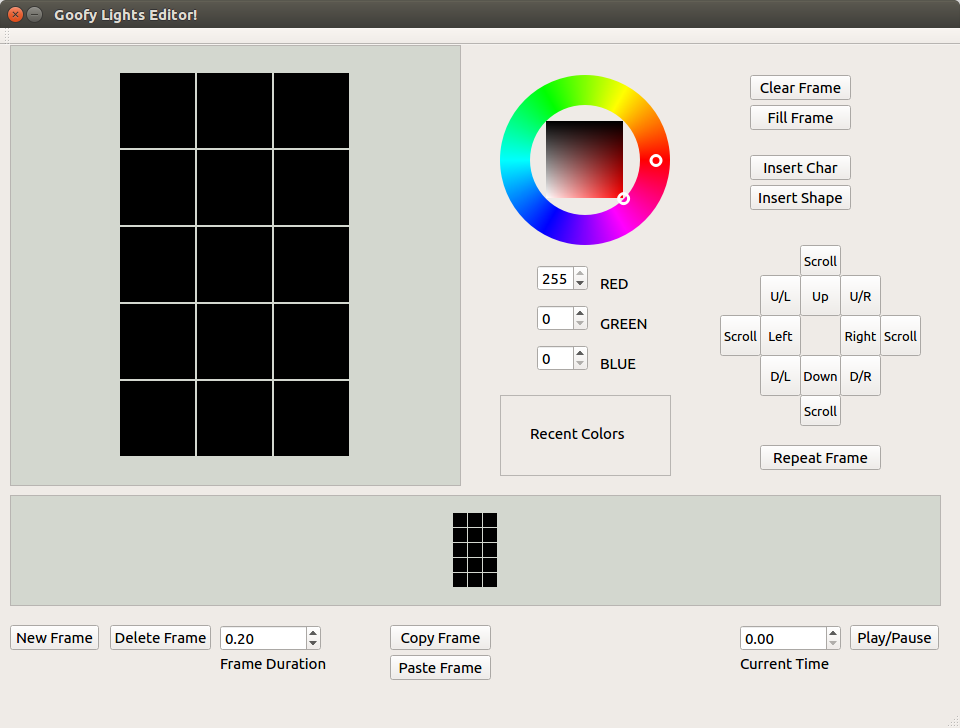
\includegraphics[width=320pt]{GUI_Screenshots/gui_5_4.png}}
  	\caption{Grid size demo 5x3}
  	\label{fig:GUI Design 5 size demo 2}
  \end{figure} 
  
  \begin{figure}[H]
  	\centering
  	\fbox{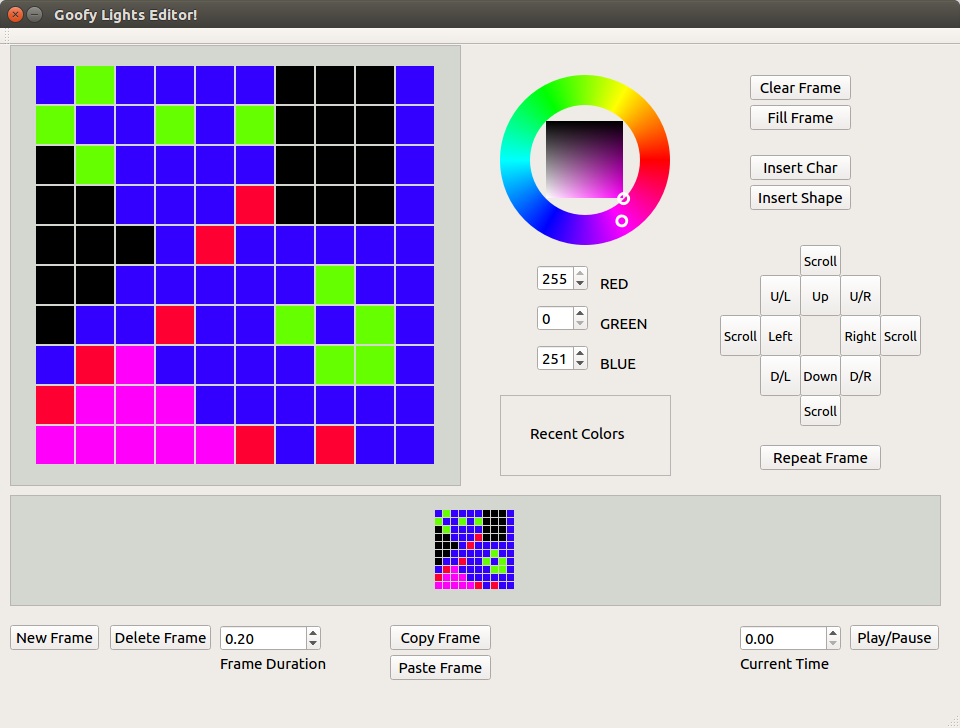
\includegraphics[width=320pt]{GUI_Screenshots/gui_5_2.png}}
  	\caption{GUI usage demo at the end of sprint 3}
  	\label{fig:GUI Design 5 demo}
  \end{figure}
  
  


\newpage
\subsubsection{UML Diagrams}

\begin{figure}[H]
	\centering
	\fbox{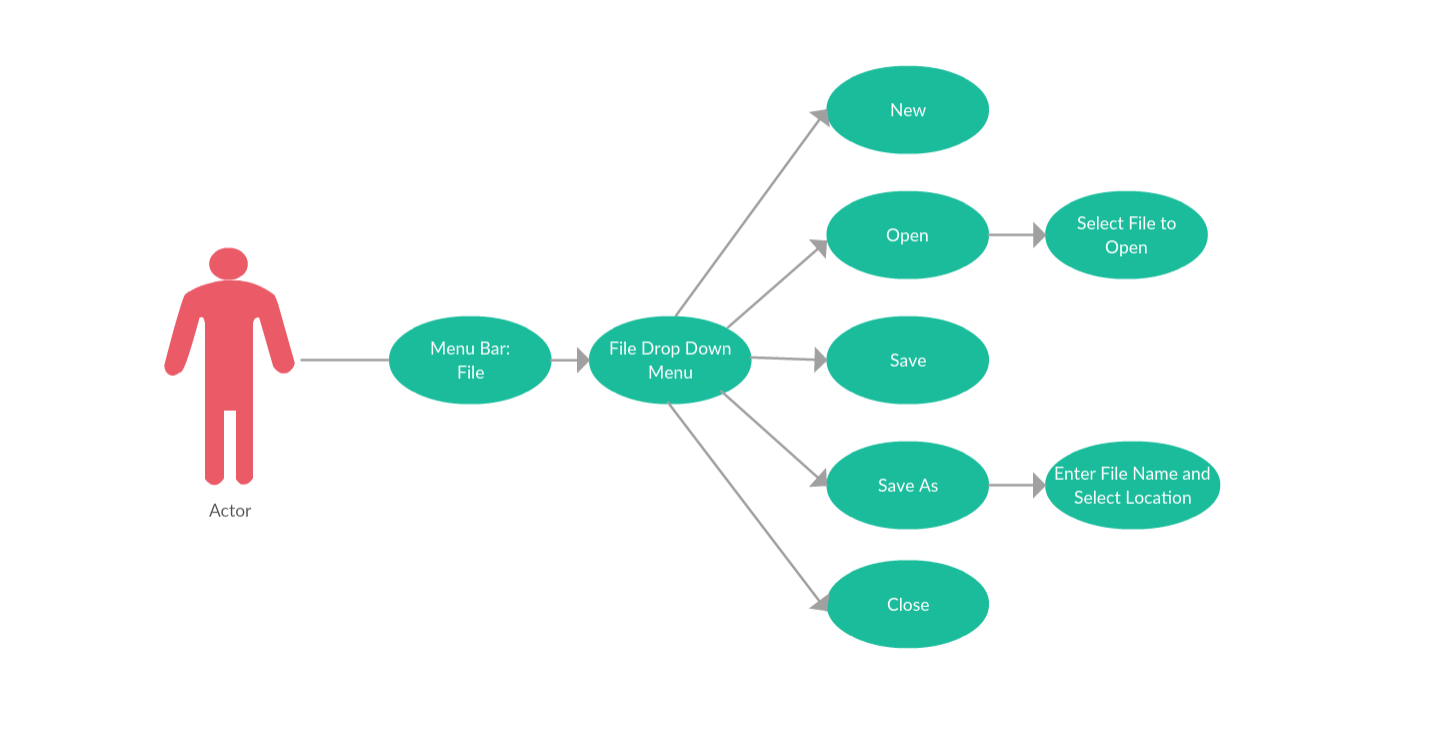
\includegraphics[width=450pt]{UML/UseCase1.png}}
	\caption{File manipulation}
	\label{fig:UC1}
\end{figure}
\begin{figure}[H]
	\centering
	\fbox{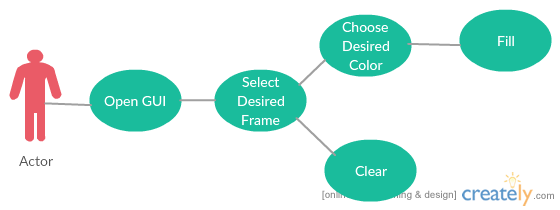
\includegraphics[width=450pt]{UML/UseCase2.png}}
	\caption{Fill or clear frame with current color}
	\label{fig:UC2}
\end{figure}
\begin{figure}[H]
	\centering
	\fbox{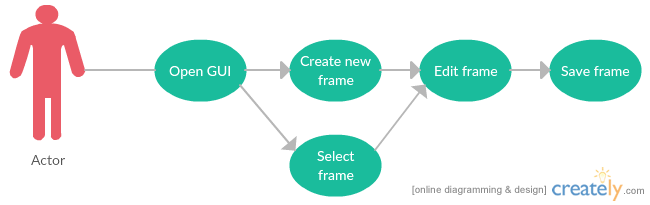
\includegraphics[width=450pt]{UML/UseCase3.png}}
	\caption{Save/copy current frame for re-use in animation}
	\label{fig:UC3}
\end{figure}

\begin{figure}[H]
	\centering
	\fbox{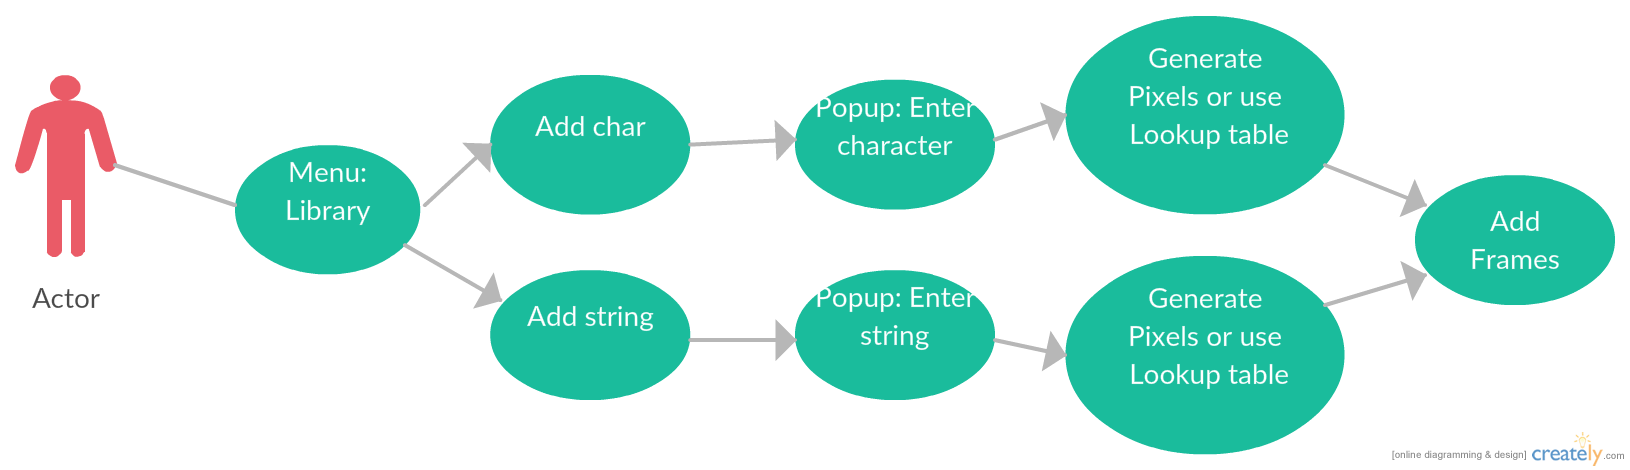
\includegraphics[width=450pt]{UML/UseCase4.png}}
	\caption{Add char/string from predefined set}
	\label{fig:UC4}
\end{figure}

\begin{figure}[H]
	\centering
	\fbox{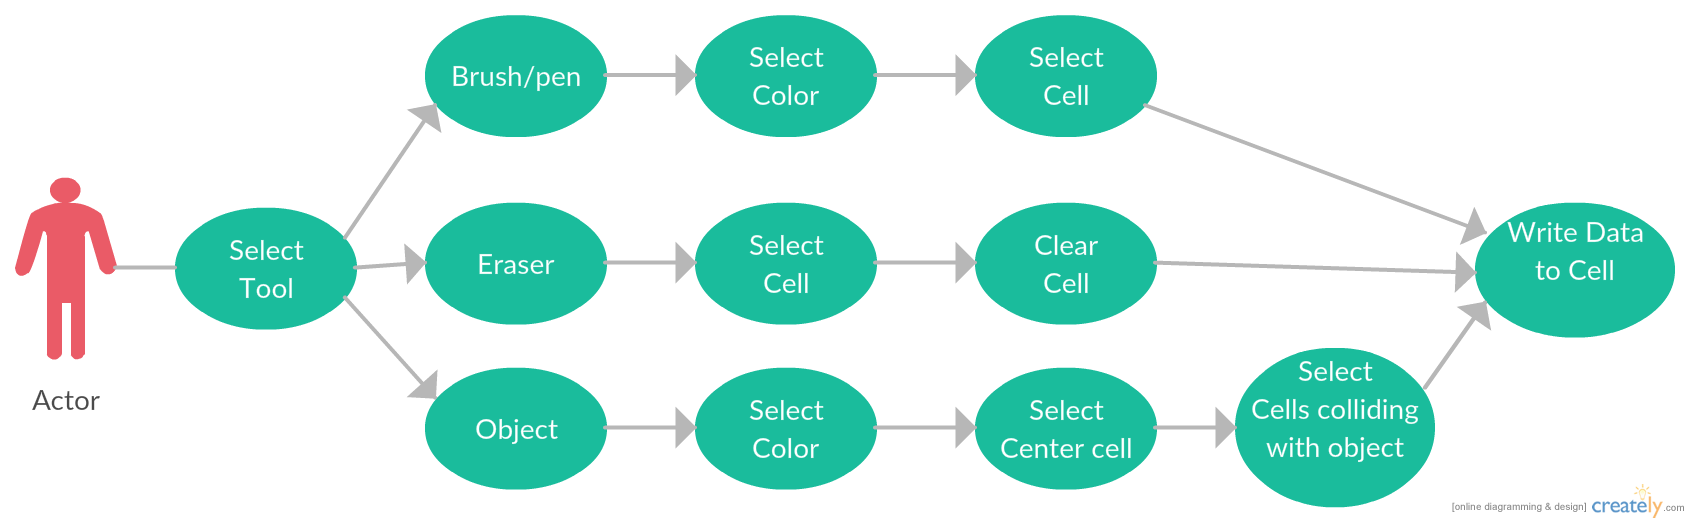
\includegraphics[width=450pt]{UML/UseCase5.png}}
	\caption{Add a pixel in any position in any color}
	\label{fig:UC5}
\end{figure}

\begin{figure}[H]
	\centering
	\fbox{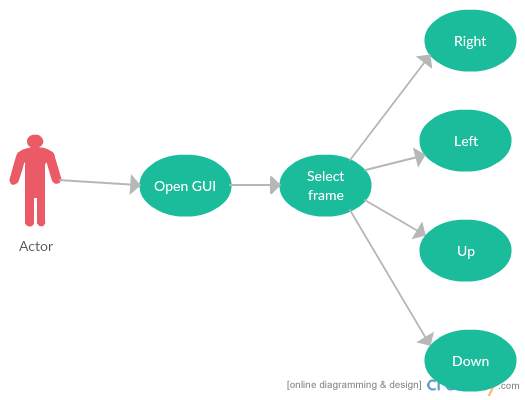
\includegraphics[width=350pt]{UML/UseCase6.png}}
	\caption{Move everything in frame 1 pixel in a direction}
	\label{fig:UC6}
\end{figure}

\begin{figure}[H]
	\centering
	\fbox{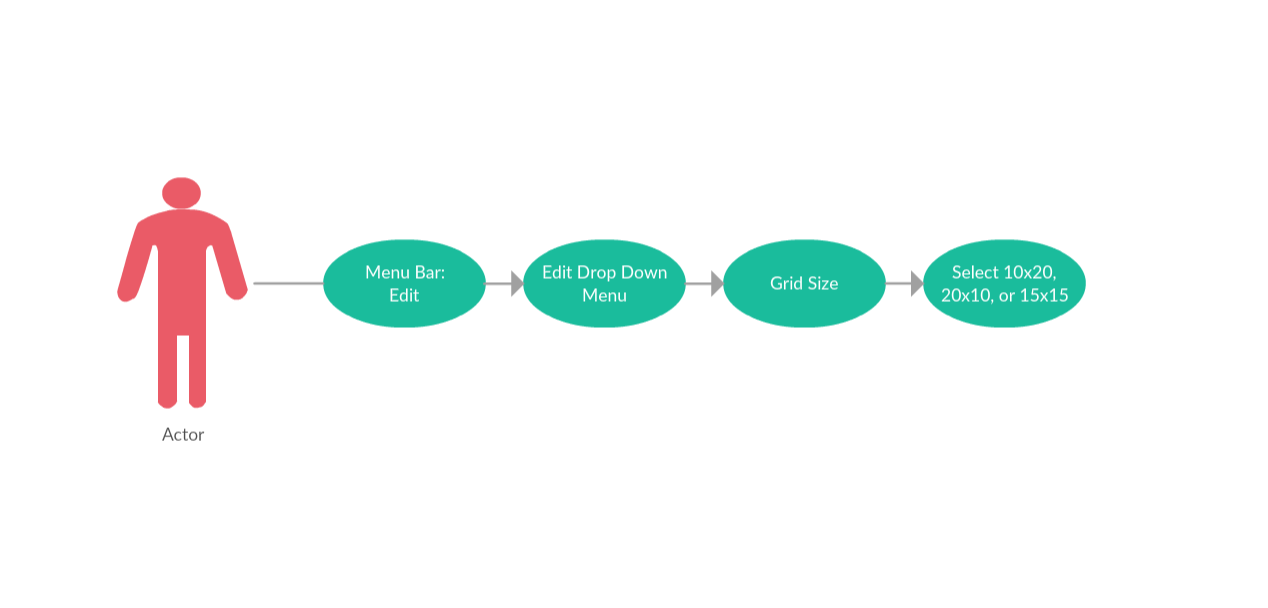
\includegraphics[width=350pt]{UML/UseCase7.png}}
	\caption{Choose grid size for the file}
	\label{fig:UC7}
\end{figure}

\begin{figure}[H]
	\centering
	\fbox{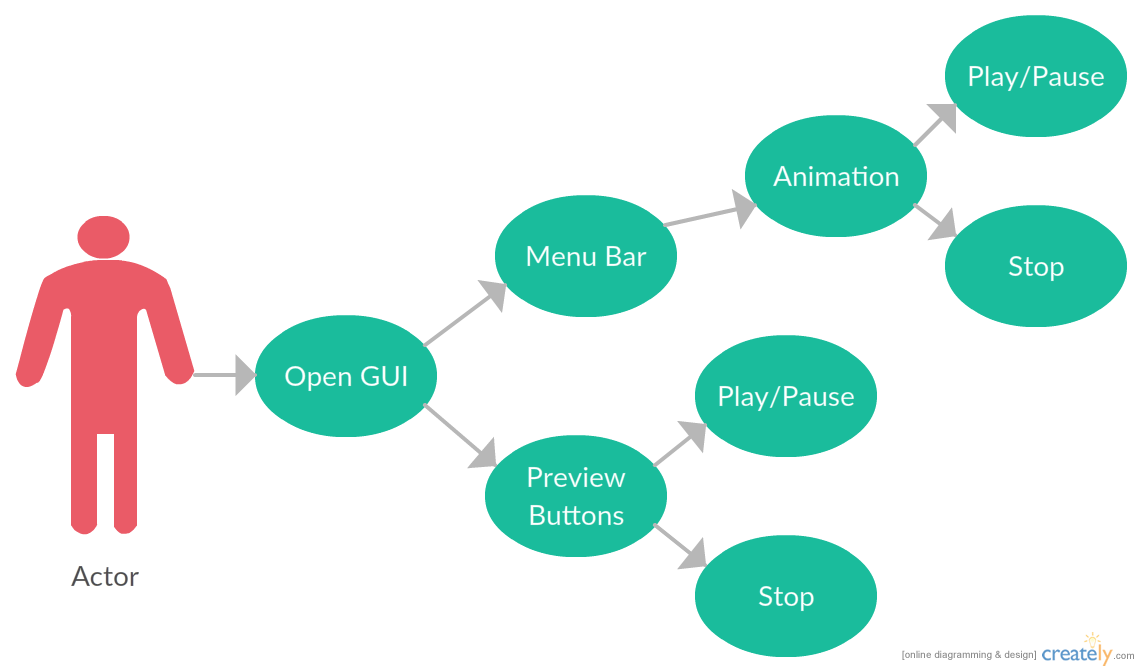
\includegraphics[width=350pt]{UML/UseCase8.png}}
	\caption{Preview play/pause/stop animation}
	\label{fig:UC8}
\end{figure}

\begin{figure}[H]
	\centering
	\fbox{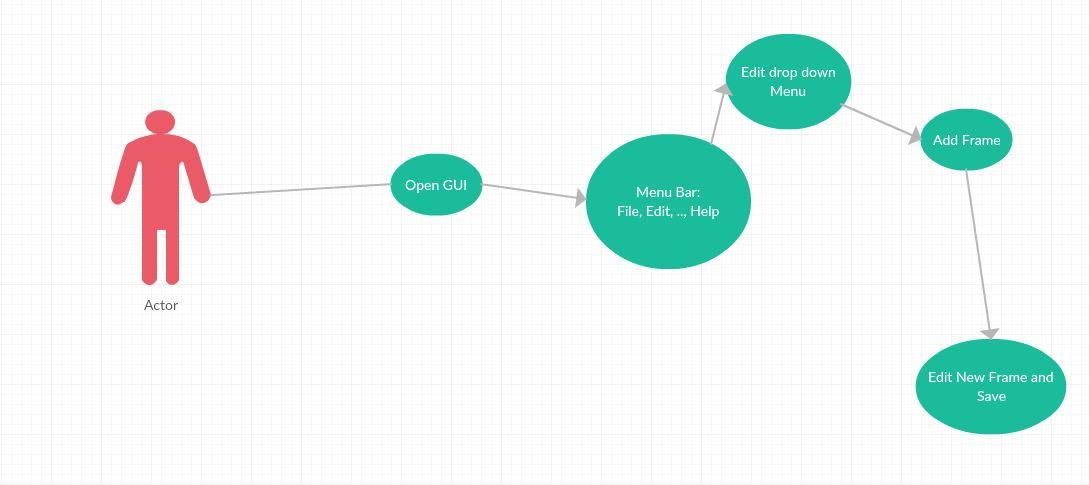
\includegraphics[width=350pt]{UML/Create_New_Frame.jpg}}
	\caption{Create new frame}
	\label{fig:UC9}
\end{figure}

\begin{figure}[H]
	\centering
	\fbox{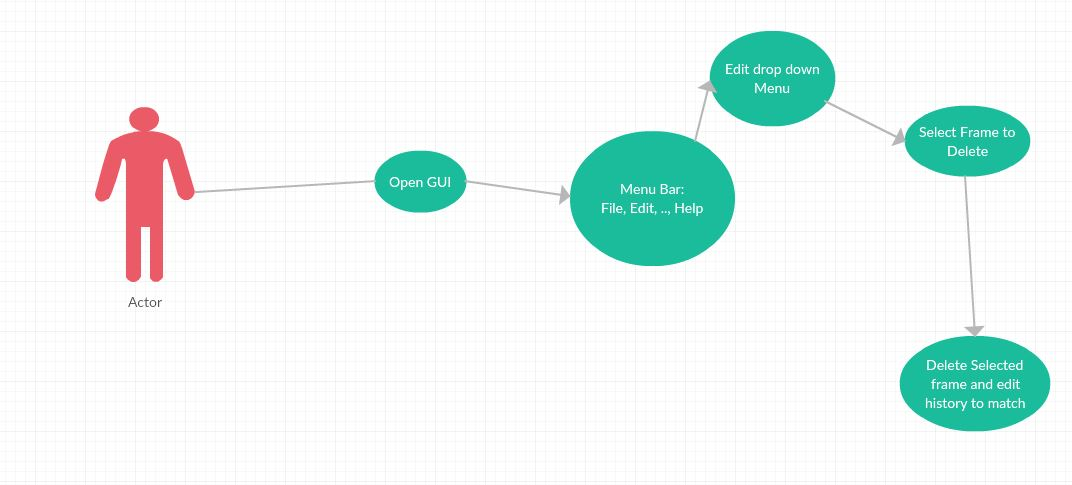
\includegraphics[width=350pt]{UML/Delete_Frame.jpg}}
	\caption{Delete a frame}
	\label{fig:UC10}
\end{figure}

\begin{figure}[H]
	\centering
	\fbox{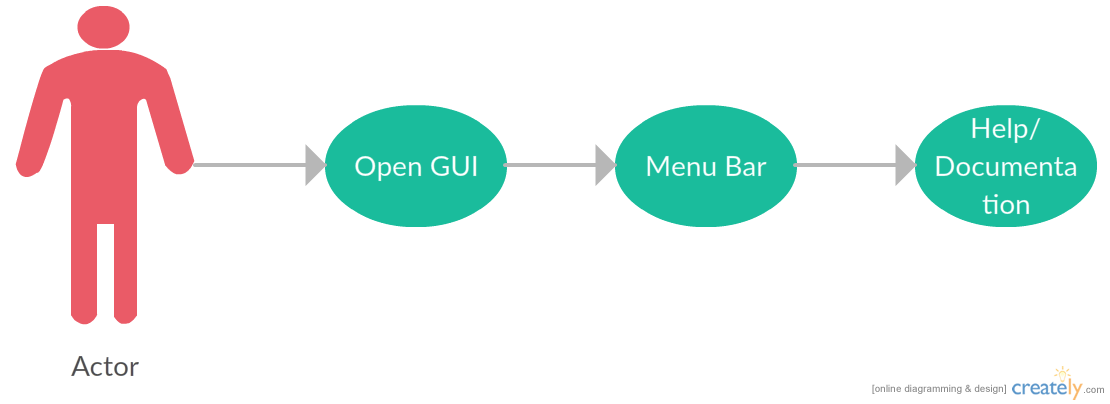
\includegraphics[width=350pt]{UML/UseCase11.png}}
	\caption{Open help/documentation text}
	\label{fig:UC11}
\end{figure}

\begin{figure}[H]
	\centering
	\fbox{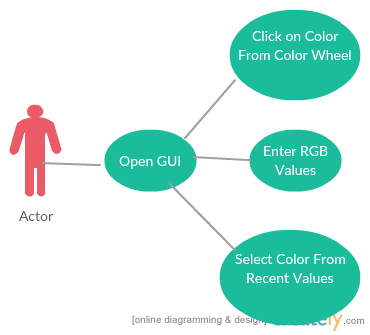
\includegraphics[width=300pt]{UML/UseCase12.png}}
	\caption{Chose a color on the colorwheel}
	\label{fig:UC12}
\end{figure}

\begin{figure}[H]
	\centering
	\fbox{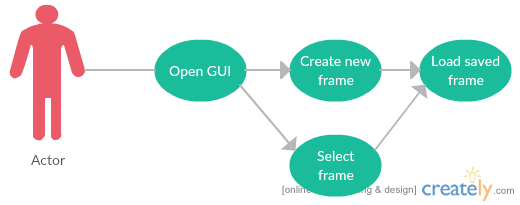
\includegraphics[width=350pt]{UML/UseCase13.png}}
	\caption{Insert a saved frame}
	\label{fig:UC13}
\end{figure}

\begin{figure}[H]
	\centering
	\fbox{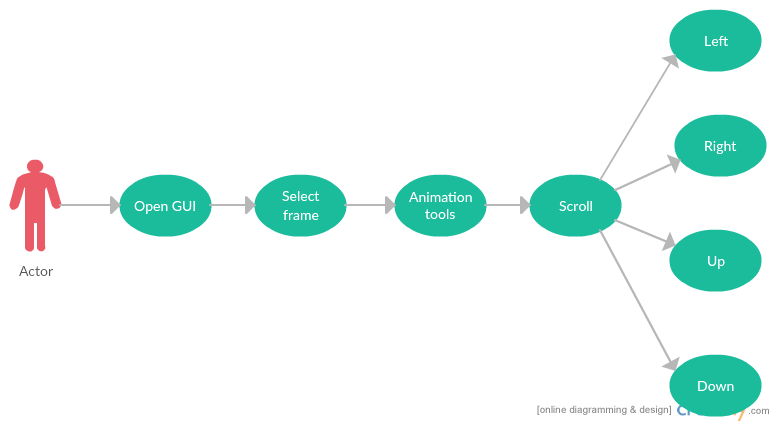
\includegraphics[width=500pt]{UML/UseCase14.png}}
	\caption{Scroll everything across entire frame}
	\label{fig:UC14}
\end{figure}

\newpage
\subsection{Timeline sprint 2}
% the language={} disables language colorings
\lstinputlisting[language={}]{Timeline_sprint_2.txt}

\newpage
\subsection{GitLog during sprint 2}
Git log since 2017\-03\-30
\lstinputlisting[language={}]{gitLog_sprint_2.log}

\newpage
\section{Sprint 3}

\subsection{Work done and problems encountered}
For this sprint in out Goofy Lights Editor we covered a lot of needed basic functionality additions, as well as resolved some issues we created with sprint 2, the summary of these changes can be found below. The main additions our group added to the Goofy Lights Editor in sprint 3, were mostly related to the changes in scope of our variables from local to global, and adding our time line to the GUI. Paul did most of the work for the addition of the time line, and it's .functionality. After we had a working time line, we added extra functionality to some of the pre-existing button we already had displayed in our GUI. This allowed us to test our new time line multiple times for correctness. We did run into a small issue with figuring out how to go about adding and updating the time line frames to match the grid that is currently being edited. A few of our team members set up a "code review" for some needed clarification on some of the GUI functions, as well as discussed how to fix the small issue with the time line mentioned above. The only other major issue we ran into this sprint, that was carried over from sprint 2, was scoping changes. We changed a lot of our local variables that were being used in multiple functions to a global scope for ease of access.

\subsection{Timeline sprint 3}
% the language={} disables language colorings
%\lstinputlisting[language={}]{Timeline_sprint_3.txt}
Our time line for sprint 3 has almost stayed the same since the last sprint. 
Original sprint 3 time line:
Solidify GUI Layout (buttons, sliders, sizes, ect.)\\

\noindent Updated Sprint 3 time line:\\
\indent Recent Color Palette \\
\indent Alter adding to the time line (linked list)\\
\indent Integration of existing code into GUI\\

\newpage
\subsection{Sprint 3 figures}
Gui Screenshots

\subsubsection{Sprint 3 GUI images}

  \begin{figure}[H]
  	\centering
  	%\fbox{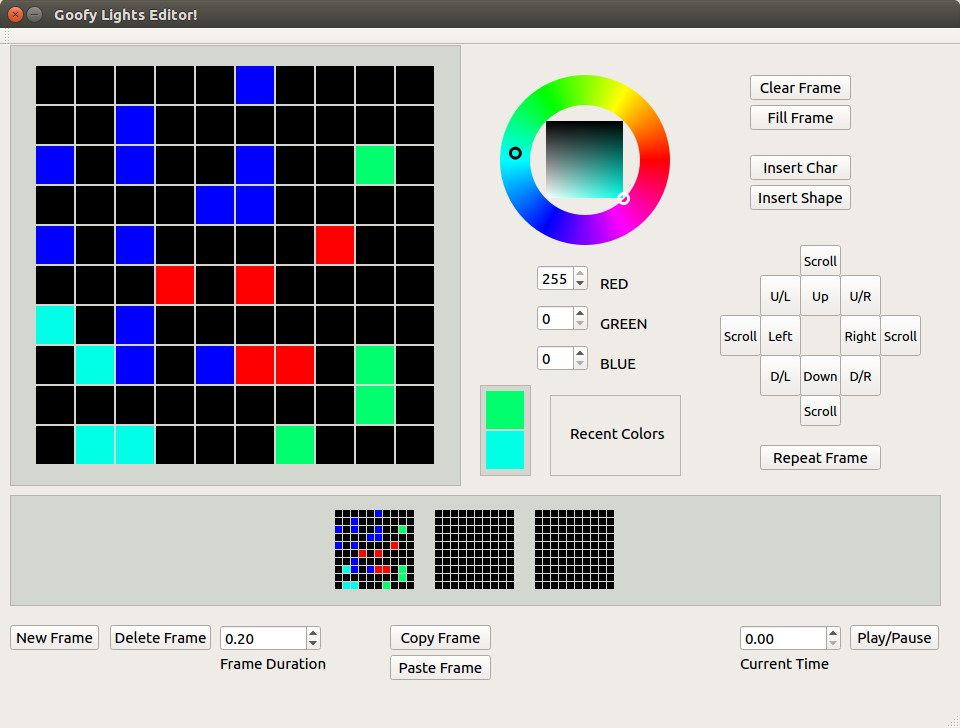
\includegraphics[width=320pt]{GUI_Screenshots/timeline.png}}
  	\caption{GUI Layout, beginning of sprint 3}
  	\label{fig:GUI Design Start Sprint 3}
  \end{figure}
  
    \begin{figure}[H]
  	\centering
  	%\fbox{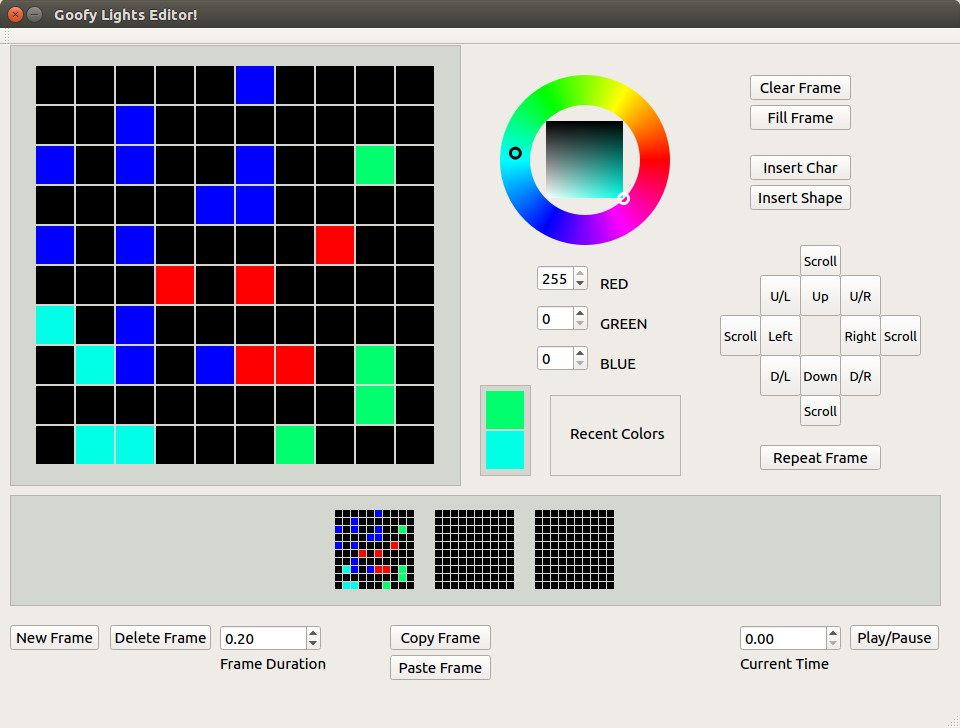
\includegraphics[width=320pt]{GUI_Screenshots/timeline.png}}
  	\caption{GUI Layout, beginning of sprint 3}
  	\label{fig:GUI Design Start Sprint 3}
  \end{figure}

\newpage
\subsection{GitLog during sprint 3}
Git log since April 11th, 2017
%\lstinputlisting[language={}]{gitLog_sprint_3.log}


\iffalse %Acts like a block comment
	\newpage
	\section{Files}
	\subsection{main.cpp file}
	\lstinputlisting{../GoofyLightsEditor/main.cpp}

	\newpage
	\subsection{FrameList.h file}
	\lstinputlisting{../GoofyLightsEditor/FrameList.h}
	\newpage
	\subsection{FrameList.cpp file}
	\lstinputlisting{../GoofyLightsEditor/FrameList.cpp}

	\newpage
	\subsection{FrameManipulation.h file}
	\lstinputlisting{../GoofyLightsEditor/FrameManipulation.h}
	\newpage
	\subsection{FrameManipulation.cpp file}
	\lstinputlisting{../GoofyLightsEditor/FrameManipulation.cpp}
\fi %end of if block acting like a block comment


\end{document}
